\section{Data driven method to estimate Charge Mis-Identification (Type-I)}
\label{sec:chargemisid}

The goal of the method is to predict, in a data driven way, the charge 
mis-identification of the electrons. This is accomplished
by measuring ``Charge-flip Rate'', $P_{ChargeFlip}$ using the Drell-Yan sample within the Z mass region
($76 < m_{ee} < 106 $ GeV). 

\subsection{Description of Charge-flip rate}

The method uses the probability of an electron to be reconstructed 
with a wrong charge as function of its $p_T$ and $\eta$.

\begin{equation}
P_{ChargeFlip} = \frac{N_{Wrong}(P_T, \eta)}{N_{Total}(P_T, \eta)}
\end{equation}

where $N_{Wrong}(P_T, \eta)$ is the number of wrongly charged electrons  and $N_{Total}(P_T, \eta)$ is 
the total number of electrons in the sample. We select events with same sign $(SS)$ 
and opposite sign $(OS)$ dielectrons within the $Z$ mass range, with both electrons passing the 
selection described in sections~\ref{sec:electron} and~\ref{sec:gsfctf}. 

The number of wrongly charged electrons in the barrel part of the detector can be obtained:

\begin{equation}
  N_{Wrong}(P_T, \eta) = SS(P_T, \eta) - k(P_T, \eta) * OS(P_T, \eta) 
\end{equation}

The normalization $k(P_T, \eta)$ is given by the ratio of doubly charged $SS_{++/--}$ electrons to the 
admixture of a distribution of correctly charge-identified electrons and incorrectly-charge 
identified $OS$ electrons. Once we obtain the $P_{ChargeFlip}$ in the barrel, the procedure is to use
the $P^{barrel}_{ChargeFlip}$ to obtain the rate for the endcap. The details of the procedure can be found 
in Ref.~\cite{chargefake}. 


The Charge-flip rate obtained using the $Z$ sample has limited coverage in $p_T$ and $\eta$ with respect
to the phase space covered by the \ttbar events. In order to extrapolate to the $p_T$ and $\eta$ 
range covered by the \ttbar decays, we use a large ``electron gun'' MC. The Charge-flip rate is determined 
for the MC sample. The distribution is then validated using the data driven method.

\begin{figure}[htb]
\begin{center}
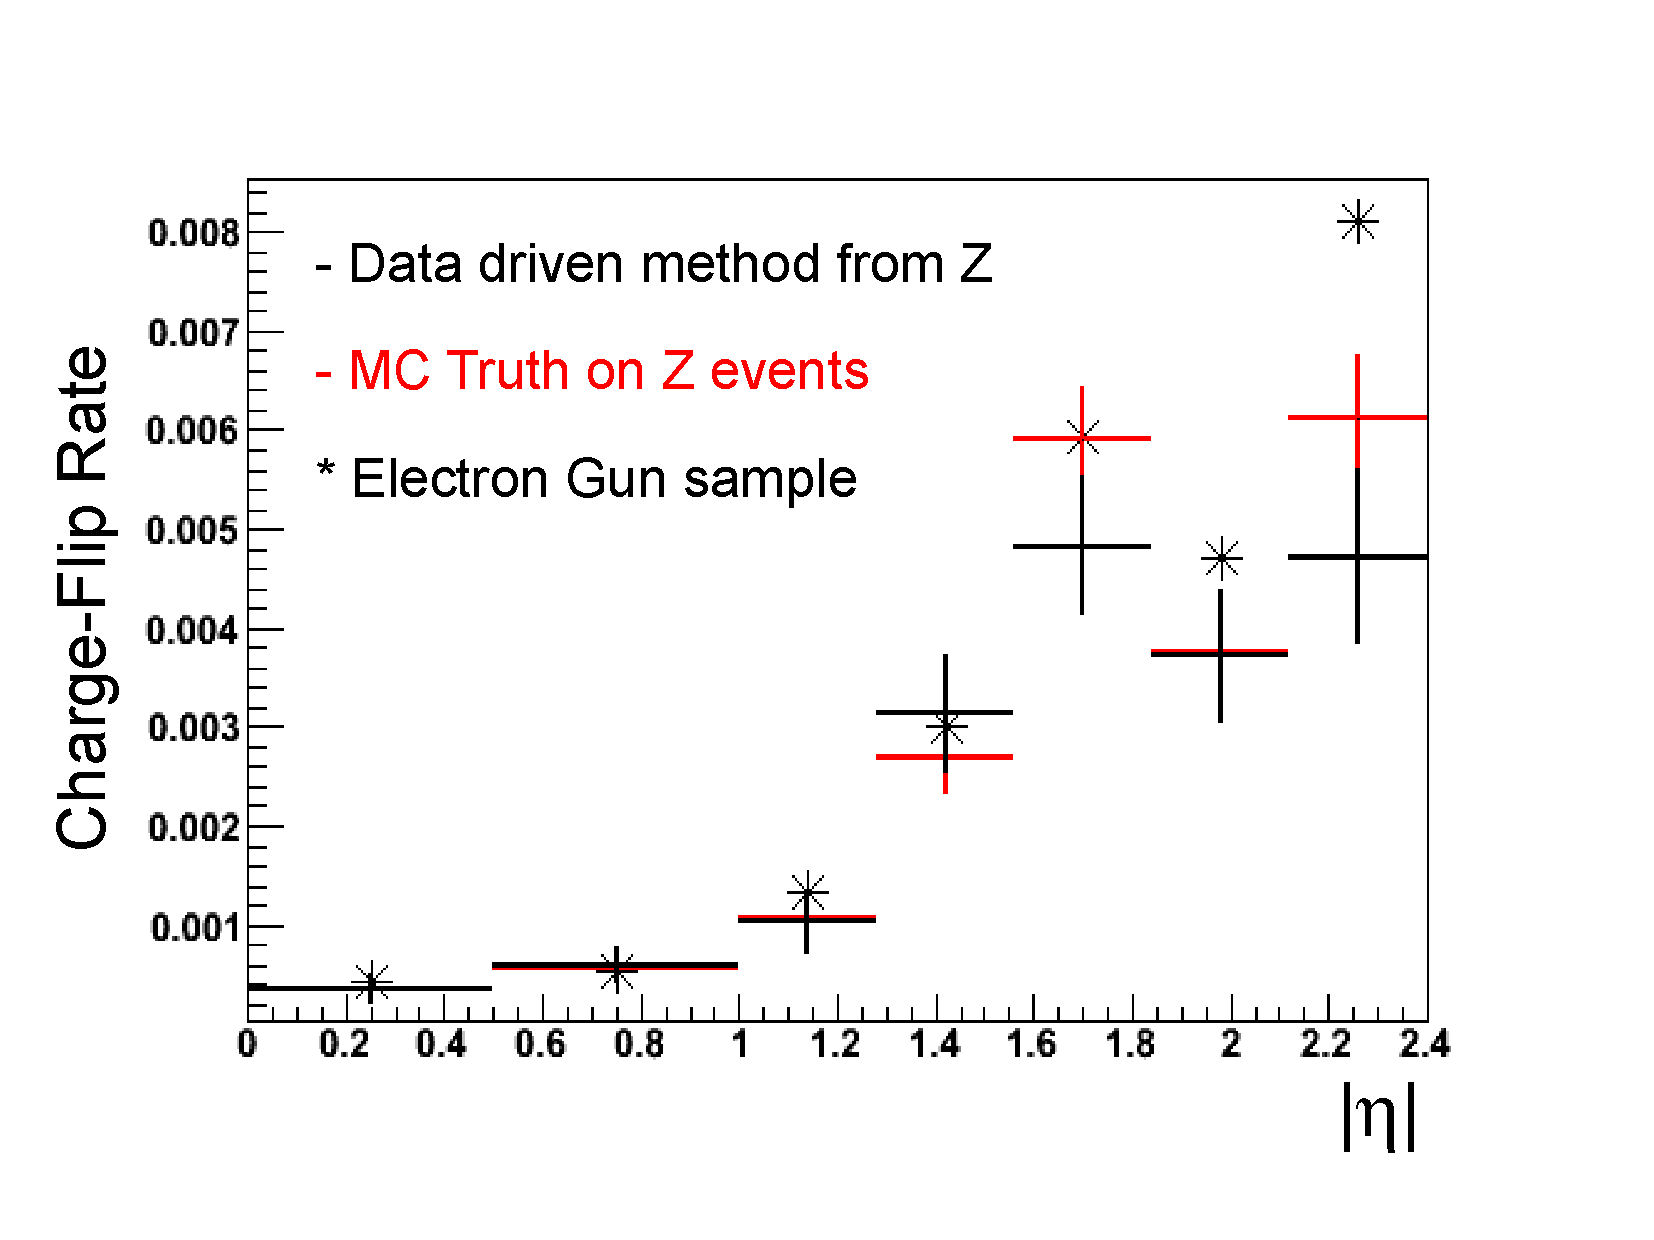
\includegraphics[width=0.7\linewidth]{figs/fr_rate.pdf}
\caption{Charge-flip rate as a function $|\eta|$ for the ``electron gun'' sample (star) compared with 
distributions using data driven method from $Z$ (black histograms) as well as truth matched $Z$ events 
(red histogram).\label{fig:charge_fliprate}}
\end{center}
\end{figure}

Figure~\ref{fig:charge_fliprate} shows the charge-flip rate as a function of $|\eta|$. The distribution from 
the ``electron gun'' sample agrees well with the expectation from data driven method
using $Z$ as well as MC truth matched $Z$ events. It should be noted that the charge-flip rate roughly 
reproduces the Charge mis-identification rate we observed earlier in Figure~\ref{fig:charge_misid} a).

\subsection{Application of Charge-flip rate to our analysis}

We now perform a rate test on \ttbar MC events by relaxing cuts on \met and jets. The test is meant
to demonstrate that the Charge-flip rate as determined from the ``electron gun'' sample can be applied
to \ttbar events. Dilepton events are selected without any \met and jet cuts using an integrated 
luminosity of 100 pb$^{-1}$. The observed event yield is obtained by selecting same sign electrons events.
In order to get the estimation we use the following procedure:

\begin{itemize}
\item Select opposite sign dielectrons using the standard selection.
\item Obtain the $P^1_{ChargeFlip}$ and  $P^2_{ChargeFlip}$ for each electron for a given $p_T$ and $\eta$.
\item Assuming either of the electrons can flip signs, the flip probability is given by $ F = P_{ChargeFlip}/(1 - P_{ChargeFlip})$.
\item Weight each event by $weight * (F^1 + F^2)$.
\item Add up all of the weights
\end{itemize} 
Results of the Monte Carlo tests for event yields is given in Tables~\ref{tab:ChFlip_Test}. From this study we 
can conclude that the Charge-flip rate does a very good job of reproducing the rate of charge mis-identification
of electrons in \ttbar events.  
\begin{table}[hbt]
\begin{center}
\begin{tabular}{|l|c|}\hline
Sample & Event yield \\ \hline
\ttbar (Observed) & 2.4 $\pm$ 0.3 \\
\ttbar (Predicted) & 2.1 \\
\hline
\end{tabular}
\caption{ Monte Carlo test of the electron Charge-flip rate.  Rates are normalized to 100 pb$^{-1}$ of integrated luminosity. \label{tab:ChFlip_Test}}
\end{center}
\end{table}

We are now ready to apply the Charge-flip rate to our \ttbar sample. The same sign dilepton sample will have 
three different contributions from Type-I, Type-II and Type-III events. The results of the application of 
the procedure outlined above is summarized in Table~\ref{tab:ChFakePredict}.
\vspace{2mm}
\begin{table}[hbt]
\begin{center}
\begin{tabular}{|l|c|c|c|c|c|c|}\hline
Same Sign leptons & Total &      Type-I &  Type-II & Type-II a) & Type-II b) & Type-III \\ \hline
$ee$ (predicted) 	 & 0.05 & 	0.05 &	0.00 &	0.00 &	0.00 &	0.00 \\
$\mu\mu$ (predicted)     & 0.00 &	0.00 &	0.00 &	0.00 &	0.00 &	0.00 \\
$e\mu$ (predicted)	 & 0.07 &	0.07 &	0.00 &	0.00 &	0.00 &	0.00 \\
total (predicted) 	 & 0.12 &	0.12 &	0.00 &	0.00 &	0.00 &	0.00 \\
\hline
\end{tabular}
\caption{ The number of events predicted using Charge-flip rate in \ttbar events for various types. Rates are normalized 
to 100 pb$^{-1}$.\label{tab:ChFakePredict}}
\end{center}
\end{table}

Using Table~\ref{tab:fakeOrigin} as observed and Table~\ref{tab:ChFakePredict} as the 
prediction, we find that the Charge-flip method predicts the bulk of the Type-I events. As expected,
the method does not predict any contribution from Type-II events. 
We consider the agreement to be satisfactory.
%This is quite satisfactory
%assuming a large systematic uncertainty are involved on these predictions.

